\documentclass[a4paper, 9pt]{extarticle}

\usepackage[utf8]{inputenc}
\usepackage[spanish]{babel}
\usepackage{geometry}
\usepackage{graphicx}
\usepackage{float}
\usepackage{booktabs}
\usepackage{amsmath}
\usepackage{hyperref}

\geometry{
    top=2cm,
    bottom=2cm,
    left=2.5cm,
    right=2.5cm
}

\title{\vspace{-1.5cm} {\Large\bfseries Física Computacional: Evaluación Práctica} -- \large Prueba 2A: Doomscrolling}
\author{\normalsize Íñigo Aliod (Ilakyyyy) -- 924640}
\date{\normalsize\today}

\begin{document}

\maketitle
\thispagestyle{empty}

\section{Introducción}
Se nos plantea decidir cuál es mejor opción: la linterna circular, o la linterna cónica.
Para ayudar a extraer una conclusión, disponemos de la función ``Extract information'', que genera
un par de resultados por NIP; uno con la linterna circular, y otro con la linterna cónica.
Dichos resultados contienen el número de preguntas realizadas $(10-p)$, donde $p$ son los profesores
restantes, la distancia $d$ recorrida por el estudiante, y la duración de la simulación, $t$.

En base a esto, parece razonable considerar que el mejor tipo de linterna será aquel con 
mayor número de preguntas realizadas, lo que se debería corresponder (para poder considerarlo válido) tanto con 
una mayor distancia recorrida, como con una mayor duración de la simulación.

Dado que disponemos de 115 datos para cada tipo de linterna, parece razonable también el considerar 
que es un tamaño de muestra suficiente para hacer esta estadística

\section{Análisis de Datos}
A partir de los datos localizados en ``results/summary.csv'', podemos calcular las medias de las preguntas
realizadas según el área de detección, obteniendo:
$${q_{asked, cone}} = 3 \quad {q_{asked, circle}} = 2$$
Podemos incluso ir más lejos, y utilizar RCommander para hacer un histograma de frecuencias de 
las preguntas hechas, según la forma del área de detección; así como para hacer
un diagrama de cajas (y bigotes) de la duración de la simulación, $t$, discriminando según la 
forma de detección (un círculo o un cono), obteniendo las dos siguientes imágenes\footnote{Hechas por Eneko,
a mí no me dejaba importar el .csv en RCommander xd}:
\begin{figure}[H]
    \centering
    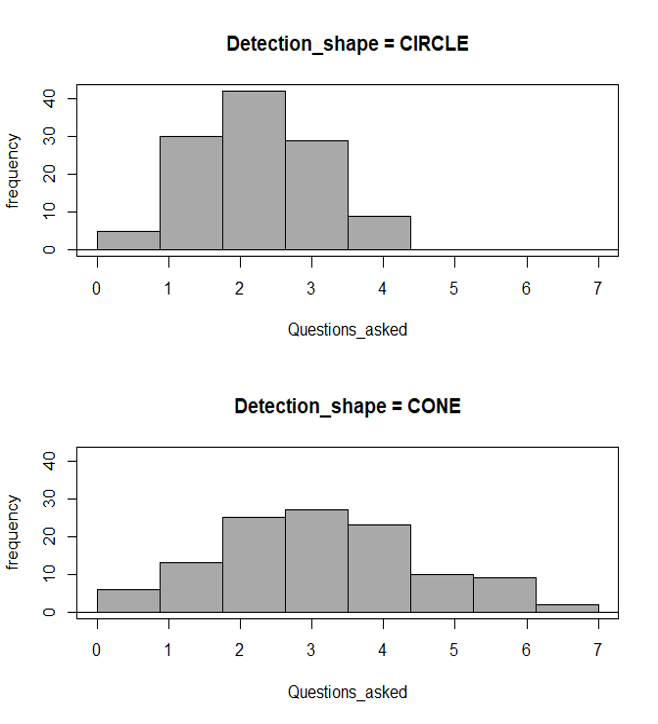
\includegraphics[width=0.4\linewidth]{Histogramas.png}
    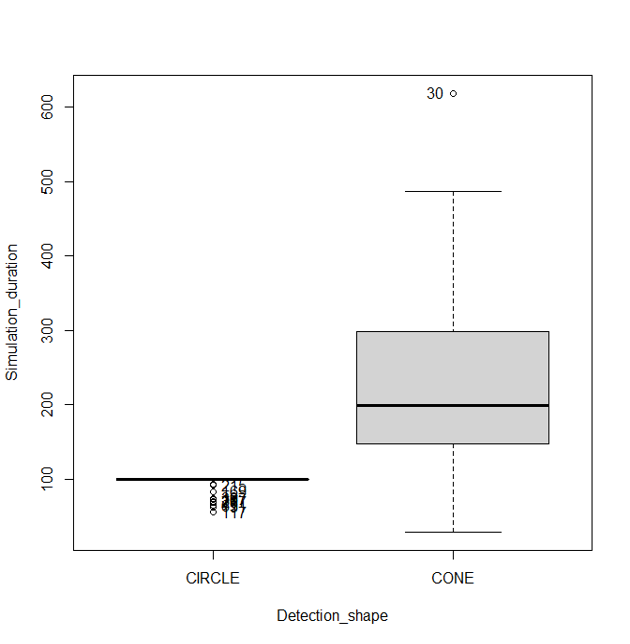
\includegraphics[width=0.4\linewidth]{CajasyBigotes.png}
\end{figure}


\section{Conclusión}
A la vista de las gráficas anteriores, podemos afirmar que utilizar la forma de \textbf{cono} es 
notoriamente superior a utilizar un círculo.

Esto se debe a que, tal y como se aprecia en el diagrama de cajas, si se utiliza el círculo,
tanto la mediana como el rango intercuartílico colapsan en el valor de $t=100$s\footnote{Salvo algún 
dato atípico que se encuentra por debajo}, mientras que la mediana para el cono es de unos $t=200$s,
situándose la frontera del primer cuartil notoriamente por encima de los $100$s del círculo.

Considerando que el consumo de batería del móvil es directamente proporcional al área iluminada, 
esto resulta completamente lógico y predecible. El área iluminada por la linterna circular ($\pi r_{detection}^2$) 
es considerablemente mayor que la del sector circular que proyecta la linterna cónica. 
Al iluminar una superficie menor, el cono minimiza drásticamente el consumo de batería, permitiendo al estudiante 
mantener la luz encendida por un tiempo mucho mayor. 
Esta prolongación en la vida de la batería es lo que justifica la mayor duración de la simulación 
observada en los datos, lo que se traduce directamente en un aumento significativo de las oportunidades 
del estudiante para encontrar profesores y hacer más preguntas antes de que se apague el móvil y sucumba al pánico, 
tal y como se aprecia en los histogramas.
\end{document}